% Figure of the starter slide deck (scripts/gen-starters.ts compiles it to templates/starters/deck/figures/scattering.pdf).
% Its bounding box is fixed — 100 mm x 54 mm, the axis 84 mm x 40 mm with its corner at (12 mm, 11 mm) — so
% that the deck can place its callouts over the curve by data coordinates (scripts/starters-src/deck.ts).
\documentclass[border=0pt]{standalone}
\usepackage[T1]{fontenc}
\usepackage[sfdefault]{notomath}
\usepackage{pgfplots}
\pgfplotsset{compat=1.18}
% the deck's palette
\definecolor{ink}{HTML}{222838}
\definecolor{mist}{HTML}{6E7487}
\definecolor{rule}{HTML}{E2DCD2}
% the visible spectrum, 380-760 nm: TikZ maps the middle half of a shading (25-75bp) onto the path
\definecolor{s380}{HTML}{7B4FE0}\definecolor{s440}{HTML}{3D6CF0}\definecolor{s480}{HTML}{2F9BF0}
\definecolor{s510}{HTML}{33B5A0}\definecolor{s550}{HTML}{6CC04A}\definecolor{s580}{HTML}{F5C842}
\definecolor{s610}{HTML}{F59A3B}\definecolor{s650}{HTML}{EE5E45}\definecolor{s700}{HTML}{D9443F}\definecolor{s760}{HTML}{A8323A}
\pgfdeclarehorizontalshading{spectrum}{100bp}{color(0bp)=(s380); color(25bp)=(s380); color(32.89bp)=(s440);
  color(38.16bp)=(s480); color(42.11bp)=(s510); color(47.37bp)=(s550); color(51.32bp)=(s580); color(55.26bp)=(s610);
  color(60.53bp)=(s650); color(67.11bp)=(s700); color(75bp)=(s760); color(100bp)=(s760)}
\begin{document}
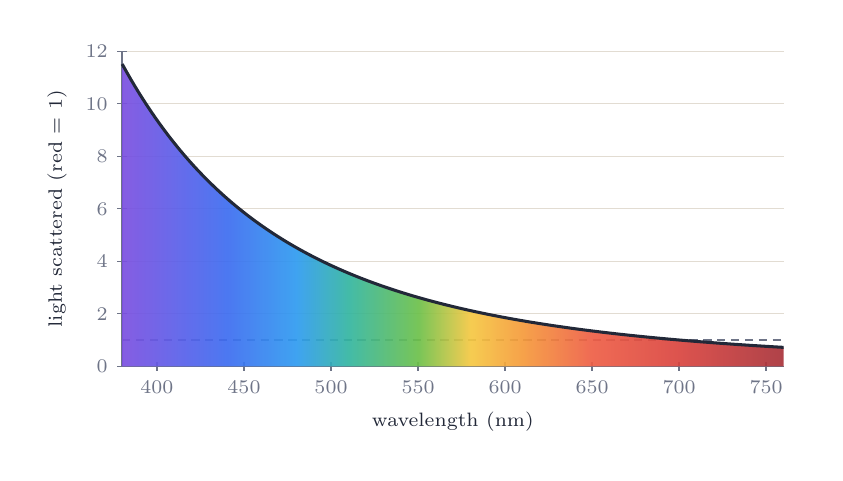
\begin{tikzpicture}
\useasboundingbox (-12mm,-11mm) rectangle (88mm,43mm);
\begin{axis}[at={(0,0)}, anchor=south west, scale only axis, width=84mm, height=40mm,
  xmin=380, xmax=760, ymin=0, ymax=12, xtick={400,450,...,750}, ytick={0,2,...,12},
  axis lines=left, axis line style={mist, line width=0.5pt, -}, major tick length=1.2mm, tick style={mist, line width=0.5pt},
  ymajorgrids, grid style={rule, line width=0.4pt},
  ticklabel style={font=\fontsize{7}{8}\selectfont, text=mist},
  label style={font=\fontsize{7.5}{9}\selectfont, text=ink},
  xlabel={wavelength (nm)}, ylabel={light scattered (red = 1)}, clip=false]
\addplot[mist, densely dashed, line width=0.5pt, domain=380:760] {1};
\addplot[draw=none, shade, shading=spectrum, opacity=0.92, domain=380:760, samples=160] {(700/x)^4} \closedcycle;
\addplot[ink, line width=1.1pt, domain=380:760, samples=160] {(700/x)^4};
\end{axis}
\end{tikzpicture}
\end{document}
